% vim:set number:
\documentclass{book}
\usepackage{amsmath,amsfonts,amssymb}
\usepackage[american]{circuitikz}
\usepackage{pgfplots}
\usepgfplotslibrary{fillbetween}
\usetikzlibrary{arrows.meta, calc, intersections, patterns}

\pgfplotsset{compat=1.13}

\tikzset{%
    sec/.style={line width = 0.5pt},
    seca/.style={line width = 0.5pt, -{Stealth[scale width=0.7]}},
    blo/.style={rectangle,fill=white, inner sep=1.5pt},
    pri/.style={line width = 1pt},
    pria/.style={line width = 1pt, -{Stealth[scale width=0.7]}},
    secda/.style={line width=0.5pt, {Stealth[scale width=0.7]}-{Stealth[scale width=0.7]}},
    prida/.style={line width = 1pt, {Stealth[scale width=0.7]}-{Stealth[scale width=0.7]}},
}
\ctikzset{%
    bipoles/americaninductor/coil height=0.12,
    bipoles/capacitor/height=0.2,
    bipoles/capacitor/width=0.1,
    bipoles/resistor/height=0.2,
    bipoles/resistor/width=0.4,
}

\begin{document}

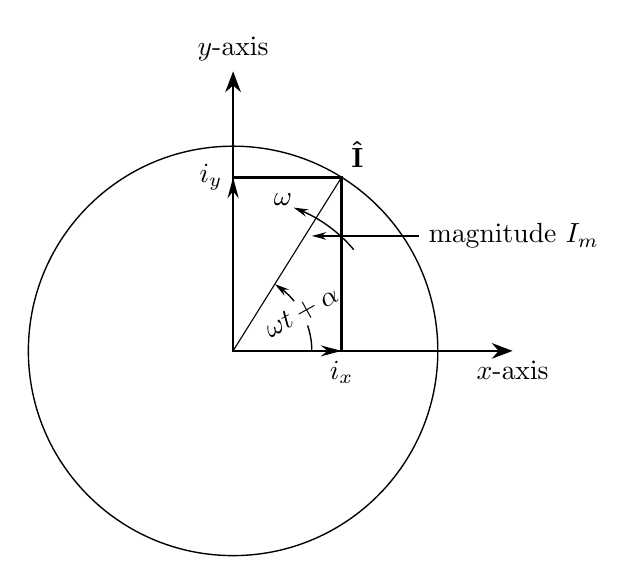
\begin{tikzpicture}
    \coordinate (A) at (58:2.6);
    \coordinate (O) at (0,0);
    \draw [seca] (O) +(0:1)arc(0:58:1)node[blo,midway,rotate=29]{$\omega t + \alpha$};
    \draw [sec](0,0)ellipse[radius=2.6];
    \draw [pri,Stealth-Stealth](0,3.55)node [anchor = south]{$y$-axis}--(0,0)--(3.55,0)node[anchor = north]{$x$-axis};
    \draw (0,0)--(A)node[anchor=south west]{$\mathbf{\hat I}$};
    \draw [pri](O|-A)--(A)--(A|-O);
    \draw [pria](O)--(O|-A)node[anchor = east]{$i_y$};
    \draw [pria](O)--(A|-O)node[anchor = north]{$i_x$};
    \draw [seca] (O)+(40:2)arc(40:70:1.8cm)node[ above left =-3pt]{$\omega$};
    \draw [seca] (2.36,1.46)node[anchor = west]{magnitude $I_m$} -- (1,1.46);
\end{tikzpicture}

%-----------------------------------
%          Figura 1.2
%-----------------------------------

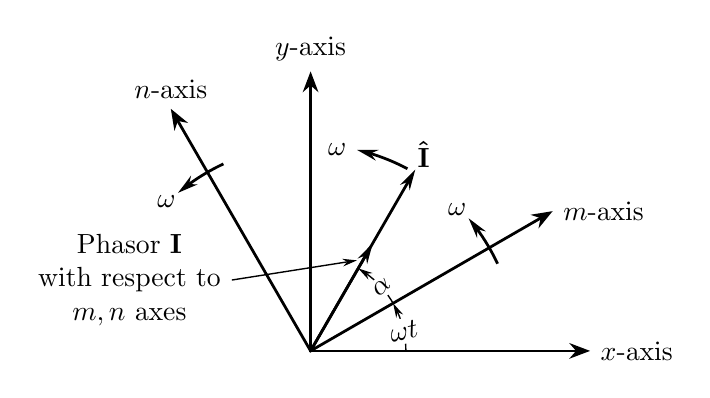
\begin{tikzpicture}
    \coordinate (O) at (0,0);
    \draw [Stealth-Stealth,line width=1pt](0,3.55)node [anchor = south]{$y$-axis}--(O)--(3.55,0)node[anchor = west]{$x$-axis};
    \draw [Stealth-Stealth,line width=1pt,rotate=30](0,3.55)node [anchor = south]{$n$-axis}--(O)--(3.55,0)node[anchor = west]{$m$-axis};
    \draw [seca] (O) +(0:1.21)arc(0:30:1.21)node[blo,pos=0.4,rotate=12]{$\omega t$};
    \draw [seca] (O) +(30:1.21)arc(30:60:1.21)node[blo,pos=0.4,rotate=42]{$\alpha$};
    \draw [pria] (O) -- (60:2.66)node[above right=-3pt]{$\mathbf{\hat I}$};
    \draw [pria] (O) -- (60:1.58);
    \draw [pria] (O) +(25:2.62) arc (25:40:2.62) node[above left=-3pt]{$\omega$};
    \draw [pria] (O) +(62:2.62) arc (62:77:2.62) node[left]{$\omega$};
    \draw [pria] (O) +(115:2.62) arc (115:130:2.62) node[below left=-3pt]{$\omega$};
    \draw [seca](-1,0.9)node[text width=2.35cm,align=center,left]{Phasor $\mathbf{I}$ \\ with respect to \\$m,n$ axes}--(0.59,1.15);
\end{tikzpicture}

%-----------------------------------
%          Figura 1.3
%-----------------------------------
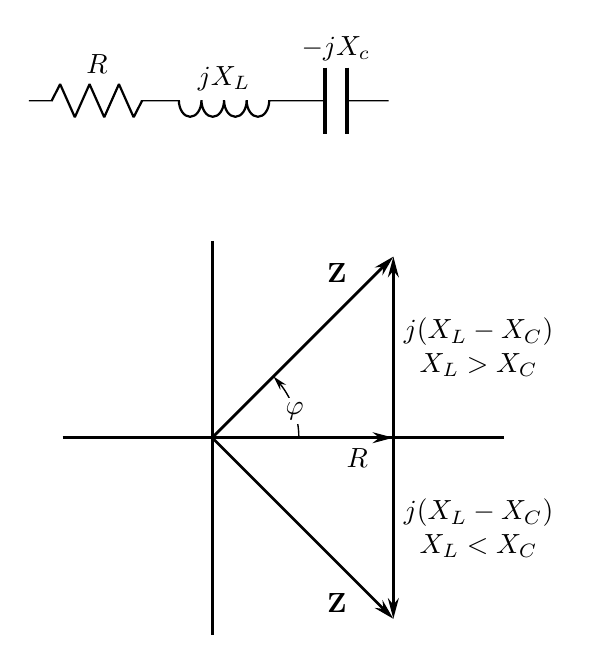
\begin{tikzpicture} %TODO corregir capacitor
    \coordinate (O) at (0,0);
    \draw (-2.33,4.28) to[R=$R$](-0.6,4.28) (0.9,4.28)to[L,l_=$jX_L$](-0.6,4.28) (0.9,4.28)to[C=$-jX_c$,thick](2.24,4.28);
    \draw [pri](-1.9,0)--(3.7,0) (0,2.5) -- (0,-2.5);
    \draw [pria](O)--(2.3,2.3)node[pos=0.8,above left]{$\mathbf{Z}$};
    \draw [pria](O)--(2.3,-2.3)node[pos=0.8,below left]{$\mathbf{Z}$};
    \draw [pria](O)--(2.3,0)node[pos=0.8,below]{$R$};
    \draw [pria](2.3,0)--(2.3,2.3)node[pos=0.5,right,align=center]{$j(X_L-X_C)$\\$X_L>X_C$};
    \draw [pria](2.3,0)--(2.3,-2.3)node[pos=0.5,right,align=center]{$j(X_L-X_C)$\\$X_L<X_C$};;
    \draw [seca](O) +(0:1.1)arc(0:45:1.1)node[blo,pos=0.4]{$\varphi$};
\end{tikzpicture}

%-----------------------------------
%          Figura 1.4
%-----------------------------------
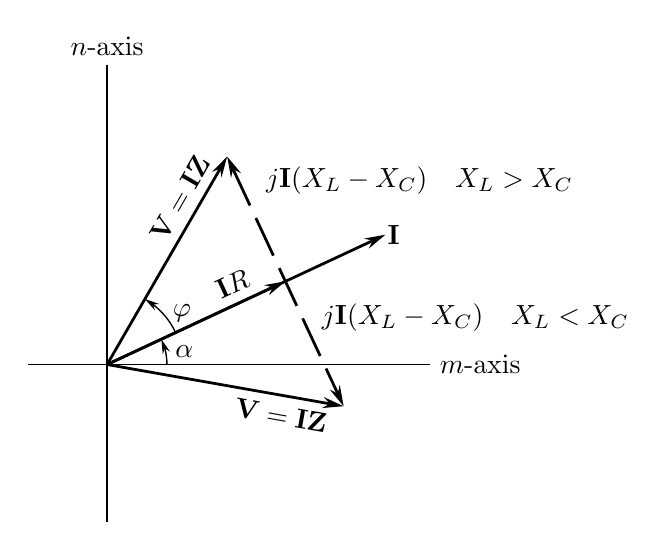
\begin{tikzpicture}
    \coordinate (a) at (25:2.5);
    \coordinate (b) at (60:3.05);
    \coordinate (c) at (-10:3.05);
    \draw [sec](-1,0) -- (4.1,0)node[right]{$m$-axis} (0,-2) -- (0,3.8)node[above]{$n$-axis};
    \draw [pria] (0,0) -- (a)node[near end,sloped,above]{$\mathbf{I}R$};
    \draw [pria] (0,0) -- (b)node[near end,sloped,above]{$\mathbf{V}=\mathbf{IZ}$};
    \draw [pria] (0,0) -- (c)node[near end,sloped,below]{$\mathbf{V}=\mathbf{IZ}$};
    \draw [pria] (0,0) -- (25:3.9)node[right=-3pt]{$\mathbf{I}$};
    \draw [prida,loosely dashed,line width=1pt,dash pattern=on 15pt off 5pt] (b) -- (c);
    \draw [seca] (0,0) +(0:0.76) arc(0:25:0.76)node[midway, right]{$\alpha$};
    \draw [seca] (0,0) +(25:0.96) arc(25:60:0.96)node[midway, right]{$\varphi$};
    \draw (2,2.14) node[above right=-3pt]{$j\mathbf{I}(X_L-X_C) \quad X_L>X_C$};
    \draw (2.71,0.4) node[above right=-3pt]{$j\mathbf{I}(X_L-X_C) \quad X_L<X_C$};
\end{tikzpicture}

%-----------------------------------
%          Figura 1.5
%-----------------------------------
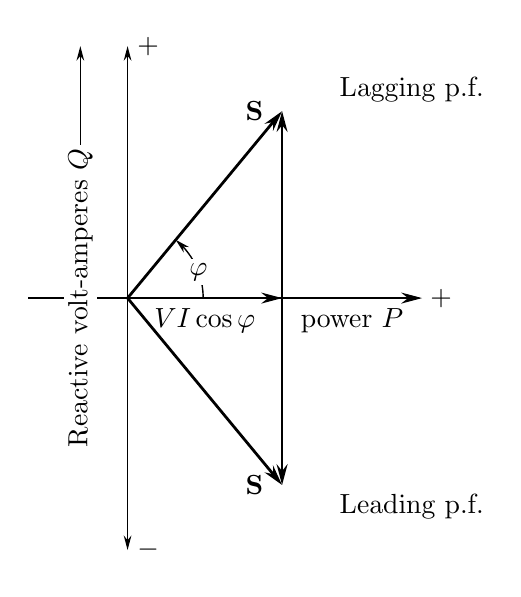
\begin{tikzpicture}
    \coordinate (O) at (0,0);
    \coordinate (a) at (50.42:3.08);
    \coordinate (b) at (-50.42:3.08);
    \draw [seca](O) +(0:0.96) arc(0:50.42:0.96)node[blo,pos=0.4]{$\varphi$};
    \draw [secda](0,3.2)node[right]{$+$} -- (0,-3.2)node[right]{$-$};
    \draw [seca](-1.26,0) -- (3.72,0)node[right]{$+$};
    \draw [pria](O) -- (a)node[left=3pt]{$\mathbf{S}$};
    \draw [pria](O) -- (b)node[left=3pt]{$\mathbf{S}$};
    \draw [pria](O) -- (a |- O)node[midway,below]{$VI\cos\varphi$};
    \draw [pria](1.96,0) -- (3.74,0)node[midway,below]{power $P$};
    \draw [seca](-0.6,1.5)--(-0.6,3.2);
    \node [blo,xshift=-0.6cm,rotate=90]{Reactive volt-amperes $Q$};
    \draw [prida](a) -- (b);
    \node at (2.57,2.37) [above right]{Lagging p.f.};
    \node at (2.57,-2.37) [below right]{Leading p.f.};
\end{tikzpicture}

%-----------------------------------
%          Figura 1.6
%-----------------------------------
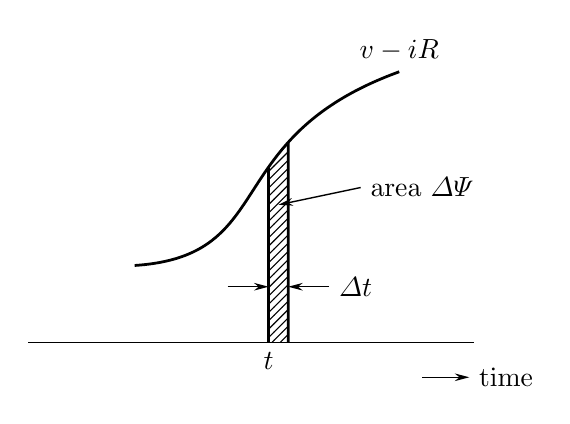
\begin{tikzpicture}
    \pgfdeclarelayer{background}
    \pgfdeclarelayer{main}
    \pgfsetlayers{background,main}
    \draw [sec] (0,0) -- (5.66,0);
    \draw [pri,name path = plot] (1.35,0.98)..controls (3.2,1.1) and (2.4,2.6)..(4.71,3.44)node[above]{$v-iR$};
    \node [below](a) at (3.05,0){$t$};
    \coordinate (b) at (3.3,0);
    \path [name path = izq](a) -- (3.05,3);
    \path [name path = der](b) -- (3.3,4);
    \path [name path = arr](0,3.44) -- (4.71,3.44);
    \draw [pri,name intersections={of=izq and plot}](a)--(intersection-1);
    \draw [pri,name intersections={of=der and plot}](b)--(intersection-1);
    \draw [seca](4.22,1.97) node[right]{area $\varDelta \varPsi$} -- (3.175,1.75);
    \draw [seca] (2.53,0.71) -- (3.05,0.71);
    \draw [seca] (3.82,0.71) node[right]{$\varDelta t$} -- (3.3,0.71);
    \draw [seca] (5,-0.44) -- (5.6,-0.44) node[right]{time};
    
    \pgfonlayer{background}
    \fill [pattern = north east lines] (3.05,0) rectangle (3.3,3);
    \fill [white,intersection segments={of=arr and plot,sequence={L* -- R*[reverse]}}];
    \endpgfonlayer
\end{tikzpicture}

%-----------------------------------
%          Figura 1.7
%-----------------------------------
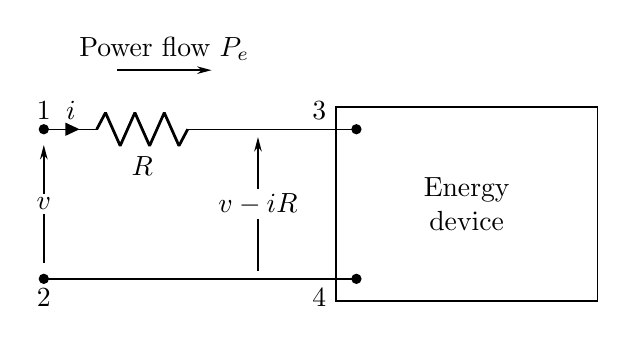
\begin{tikzpicture}
    \draw [sec] (0,0) node [below]{2} to[short,*-*] (3.97,0);
    \draw [sec] (0,1.9)node[above]{1} to[R,i>^=$i$,l_=$R$,*-](2.5,1.9) to [short,-*](3.97,1.9);
    \draw [sec] (3.71,-0.28) rectangle (7.03,2.18)node[align=center,pos=0.5]{Energy\\device};
    \draw [seca](0.93,2.65) -- (2.13,2.65) node[midway, above]{Power flow $P_e$};
    \node at (3.5,1.9) [above] {3};
    \node at (3.5,0) [below] {4};
    \draw [seca] (0,0.2)--(0,1.7)node[pos=0.5,blo]{$v$};
    \draw [seca] (2.72,0.1) -- (2.72,1.8)node[blo,pos=0.5]{$v-iR$};
\end{tikzpicture}


%-----------------------------------
%          Figura 1.8
%-----------------------------------
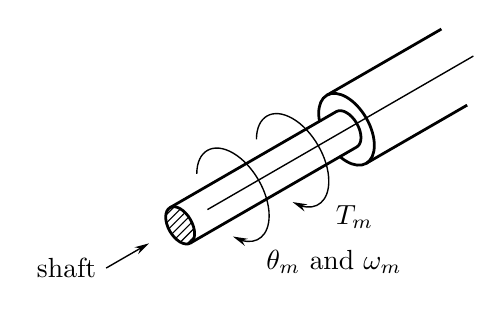
\begin{tikzpicture}
    \begin{scope}[rotate=30]
        \draw [pri] (2.44,0) ellipse [x radius =0.288, y radius = 0.5];
        \draw [pri] (2.44,-0.5) -- (3.92,-0.5) (2.44,0.5) -- (4.12,0.5);
        \filldraw [pri, fill=white] (0,-0.2595) -- (2.44, -0.2595) arc[start angle = -90, end angle = 90 , x radius = 0.15, y radius = 0.2595] -- (90:0.2595);
        \draw [pri, pattern = north east lines] (0,0) ellipse [x radius = 0.15, y radius = 0.2595];
        \draw [sec] (0.4,0) -- (4.3,0);
        \draw [seca](-1.085,0)node[left]{shaft} -- (-0.457,0);
        \path [name path = elipse1](0.775,0) ellipse[x radius = 0.375, y radius = 0.65];
        \path [name path = linea1](0.775,0)-- ++(120:0.7);
        \path [name path = elipse2](1.65,0) ellipse[x radius = 0.375, y radius = 0.65];
        \path [name path = linea2](1.65,0)-- ++(120:0.7); 
        \draw [seca, name intersections={of=elipse1 and linea1}](intersection-1) arc[start angle = 135, end angle = -135, y radius = 0.65, x radius =0.375]node[pos=0.85,below right]{$\theta_m$ and $\omega_m$};
        \draw [seca, name intersections={of=elipse2 and linea2}](intersection-1) arc[start angle = 135, end angle = -135, y radius = 0.65, x radius =0.375]node[pos=0.75, below right]{$T_m$};
    \end{scope}
\end{tikzpicture}

%-----------------------------------
%          Figura 1.9
%-----------------------------------
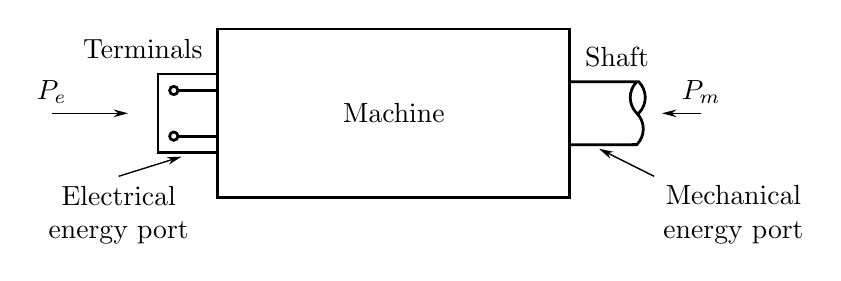
\begin{tikzpicture}
    \draw [pri](0,0.5) rectangle (0.76,-0.5);
    \draw [-{Circle[open,length=4pt,width=4pt]},pri](0.76,0.29) -- (0.13,0.29);
    \draw [-{Circle[open,length=4pt,width=4pt]},pri](0.76,-0.29) -- (0.13,-0.29);
    \draw [pri] (0.76,1.07) rectangle (5.23,-1.07) node[align=center,pos=0.5]{Machine};
    \draw [pri] (5.23,0.4) -- (6.08,0.4) arc(135:225:0.282) arc (45:-45:0.282) -- (5.23,-0.4) (6.105,0.4)arc(45:-45:0.282);
    \draw [seca](6.9,0)node[above]{$P_m$} -- (6.4,0);
    \draw [seca] (6.3,-0.8)node[below right=-0.2,align=center]{Mechanical\\energy port} -- (5.6,-0.45);
    \draw [seca](-0.5,-0.8)node[below,align=center]{Electrical\\energy port}-- (0.3,-0.55);
    \draw [seca] (-1.35,0)node[above]{$P_e$}--(-0.38,0);
    \draw node at(0.76,0.5)[above left=2pt]{Terminals};
    \draw node at(5.23,0.4)[above right=2pt]{Shaft};
\end{tikzpicture}

%-----------------------------------
%          Figura dot blank
%-----------------------------------
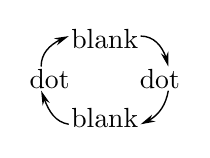
\begin{tikzpicture}[inner sep=0.7pt]
    \draw node (a) at (0,0) {dot};
    \draw node (b) at (0.7,0.5) {blank};
    \draw node (c) at (1.4,0) {dot};
    \draw node (d) at (0.7,-0.5) {blank};
    \draw [seca] (a.125) to [out=90,in=200](b.175);
    \draw [seca] (b.5) to[out=0,in=100] (c.55);
    \draw [seca] (c.305) to [out=260,in=20] (d.350);
    \draw [seca] (d.190) to [out=170,in=290] (a.235);
\end{tikzpicture}

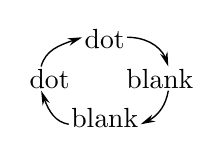
\begin{tikzpicture}[inner sep=0.7pt]
    \draw node (a) at (0,0) {dot};
    \draw node (b) at (0.7,0.5) {dot};
    \draw node (c) at (1.4,0) {blank};
    \draw node (d) at (0.7,-0.5) {blank};
    \draw [seca] (a.125) to [out=75,in=200](b.175);
    \draw [seca] (b.5) to[out=0,in=100] (c.55);
    \draw [seca] (c.305) to [out=260,in=20] (d.350);
    \draw [seca] (d.190) to [out=170,in=290] (a.235);
\end{tikzpicture}


\end{document}
